\chapter{Literature review and methodology} % Main chapter title
\label{chapter2} % For referencing the chapter elsewhere, use \ref{Chapter1}

% Define some commands to keep the formatting separated from the content
\newcommand{\keyword}[1]{\textbf{#1}}
\newcommand{\tabhead}[1]{\textbf{#1}}
\newcommand{\code}[1]{\texttt{#1}}
\newcommand{\file}[1]{\texttt{\bfseries#1}}
\newcommand{\option}[1]{\texttt{\itshape#1}}

%----------------------------------------------------------------------------------------

There are four major components to this capstone: The dataset, model training, application of XAI techniques to the trained models and evaluating the effectiveness of these XAI techniques. I provide a literature review and describe the chosen methodology of these components below.

%----------------------------------------------------------------------------------------
%	SECTION 1
%----------------------------------------------------------------------------------------
\section{Dataset: The APP-350 Corpus}
\label{app350_corpus}
The APP-350 Corpus consists of 350 annotated Android app privacy policies. Each data practice ("practice") consists of a data type and a modality. A data type describes a certain behaviour of an app that can have privacy implications (e.g. collection of a phone's device identifier or sharing of its location with ad networks). There are two modalities: \texttt{PERFORMED} (i.e. a practice is explicitly described as being performed) and \texttt{NOT\_PERFORMED} (i.e. a practice is explicitly described as not being performed). Altogether, 57 different practices were annotated. As not all practices had sufficient numbers to train models of sufficient baseline performance, I focused on training models on the top 5 practices by frequency\footnote{The performance of the models of the top $n$ frequently occurring practices is later elaborated on in Chapter~\ref{chapter4}.}. The data types and modalities that are used for the rest of the capstone are provided in Table~\ref{tab:data_practices} and ~\ref{tab:modalities}.

\begin{table}[]
	\resizebox{\textwidth}{!}{%
	\begin{tabular}{|l|p{0.8\linewidth}|}
	\hline
	\textbf{Data Type}                 & \textbf{Description}                                                                                    \\ \hline
	Contact\_E\_Mail\_Address & The policy describes collection of the user's e-mail.                                          \\ \hline
	Identifier\_Cookie\_or\_similar\_Tech & The policy describes collection of the user's HTTP cookies, flash cookies, pixel tags, or similar identifiers. \\ \hline
	Identifier\_IP\_Address   & The policy describes collection of the user's IP address.                                      \\ \hline
	Location                  & The policy describes collection of the user's unspecified location data.                       \\ \hline
	\end{tabular}%
	}
	\caption{List of top 5 data practices and their descriptions.}
	\label{tab:data_practices}
\end{table}

\begin{table}[]
	\resizebox{\textwidth}{!}{%
	\begin{tabular}{|l|p{0.8\linewidth}|}
	\hline
	\textbf{Party}                 & \textbf{Description}                                                                                    \\ \hline
	1stParty & The policy describes collection of data from the user by the app publisher.                                          \\ \hline
	3rdParty & The policy describes collection of data from the user by ad networks, analytics services, or other third parties. \\ \hline
	\end{tabular}%
	}
	\caption{List of modalities.}
	\label{tab:modalities}
\end{table}

The APP-350 Corpus was annotated and used in a broader project to train machine learning models to conduct a privacy census of 1,035,853 Android apps (\cite{zimmeck2019}). The authors downloaded the data privacy practices of all apps from the Play Store with more than 350 million installs (which totalled 247 apps) and 103 randomly selected apps with 5 million installs. In total, the researchers collected the data privacy policies of 350 apps. All 350 policies were annotated by one of the authors, a lawyer with experience in data privacy law. To ensure reliability of annotations, 2 other law students were hired to double annotate 10\% of the corpus. With a mean of Krippendorff's $\alpha = 0.78$\footnote{Krippendorff's $\alpha$ is a measure of agreement, with $\alpha > 0.8$ indicating good agreement, $0.67 <= \alpha <= 0.8$ indicating fair agreement, and $\alpha < 0.67$ indicating doubtful agreement.}, the agreement between the annotations exceeded previous similar research.

Since the focus of this capstone is to assess the explainability of XAI methods specifically within a data privacy context, this dataset was chosen as it contains real-world data privacy practices as these policies were scraped from Google PlayStore apps. Thus training XAI models on such a dataset would provide a realistic insight as to the performance of these models. APP-350 is also a labelled dataset, allowing easy validation of results. If an unlabelled dataset was used, unsupervised training would have to be conducted. The performance of such models would likely be much lower because NLP models for specific vocabulary like law are still not as sophisticated as models trained on general vocabulary. Further, there are few data privacy specific labelled datasets to begin with. 

\subsection{Data pre-processing}
The annotated privacy policies were originally in \texttt{.yml} format, with one \texttt{.yml} file containing one app data privacy policy. As explained above, each data privacy policy is labelled at both the sentence and segment level. The data was restructured from \texttt{.yml} to \texttt{.csv}, with one \texttt{.csv} file containing annotated sentences and the other containing annotated segments. By having two levels of text data for model training, this would provide another dimension to compare model performance on.

\section{NLP models and text representations}
\subsection{Literature review}
Engineering tasks for legal NLP can be categorised according to tasks such as classification (i.e. such as classifying the data practice of a sentence, which is what this capstone is about) and text generation (i.e. generating legal documents). In terms of models and word representations used for these tasks, there seems to have been two waves of models that are based off neural networks: the first includes word2vec and doc2vec which were introduced around 2014, while the second includes ELMo (Embeddings from Language Models), BERT (Bidirectional Encoder Representations from Transformers) and GPT that were introduced around and after 2017 (\cite{katz_nlp_legal}). The latter more advanced models are first trained on the text corpus to generate text representations and then fine tuned for a specific task, such as classification. As alluded to earlier, the main challenge facing NLP is capturing the contextual and semantic meaning of language in a machine-understandable way. These latter models use slightly different architectures, training data and fine tuning to capture more contextual information from the text corpus.

However, while these neural networks are undoubtedly more sophisticated, if simpler models are able to produce reasonable performance, these models should be used instead. Much depends on the complexity of the text corpus, and the engineering task that the models are made for. In the case of the APP-350 corpus, Zimmeck et al. were able to use classical machine learning models instead of neural networks to achieve reasonable performance to classify sentences according to data practices. Neural networks are contrasted with classical machine learning models that include logistic regression, decision trees, and support vector machines. Classical models are much less complex and therefore more explainable than neural networks, and require much less data to train. Given that the focus is on explainability, and in any case the APP-350 corpus is probably too limited to train neural networks\footnote{For example, BERT was trained on the whole Wikipedia (and more), while GPT-2, the second iteration of GPT, was trained on 45 terabytes of data.}, I focus only on training classical models for prediction in this capstone.

Aside from classical models for prediction, there is also another category of "classical" text representations. These are those that fall under sparse vector representation (e.g. Bag-of-Words, Tf-IDF), as compared to the more contemporary and dense vector representation mentioned above that are produced using neural networks (e.g. word2vec, BERT or GPT). These sparse vector representations are purely count based and use one-hot encoding to convert a sentence into a vector, similar to the example mentioned in Section~\ref{chap1:increasing_opacity}. For dense vector representations, unlike models used for engineering tasks which have to be trained specifically for the task, it is possible to use pre-trained vectors, and then feed these as features into a classical model. Being pre-trained, this overcomes the limitations of the dataset and computing resources. However, explainability could still be affected compared to sparse vector representation.

For the models trained on the APP-350 corpus, Zimmeck et al. used a union of Tf-IDF vectors and manually crafted features which were Boolean values indicating the presence or absence of frequently occurring keywords that occurred in each data practice. They also conducted an optional pre-processing sentence filtering step which removes a segment's sentence from further processing if the sentence does not contain keywords associated with the data practice. This improved the performance of about half their classifiers. In terms of tokenisation, they lowercased all characters, removed non-ASCII characters, did not conduct stemming, normalised whitespace and punctuation, and created unigrams and bigrams. For prediction, individual classifiers were then trained for every data practice. For all the classifications (except for four categories), they trained SVC (support vector classification) models using the scikit-learn's implementation with a linear kernel, with five-fold cross validation. For the four policy classifications, word-based rule classifiers were used instead because of the limited number of training data.

For the top 5 data practices that this capstone is concerned about, Zimmeck et al. were able to achieve F1 scores ranging from 77\% (Identifier Cookie 1st Party), 91\% (Contact Email Address 1st Party) to around 90\% for location related data practices\footnote{Not all the data practices were used in training ($n = 188$) and testing ($n = 100$) these classifiers, so there is no reference performance for some of the data practices that are used in this capstone.}.

\subsection{Methodology}
Since classical models have performed well for the APP-350 corpus as seen above, I use Zimmeck et al.'s model choice and text representation of Tf-IDF as a guide for this capstone. However, for the sake of evaluating different types of word representations, I also use a pre-trained dense vector representation, GloVe (Global Vectors). 

\subsubsection{Text representations}
I use Tf-IDF (term frequency - inverse document frequency) and GloVe as the two text representations. The idea behind Tf-IDF is that words that are frequent in a document but rare across the rest of the corpus are more important in distinguishing the document from others. The Tf-IDF metric for a word in a document is calculated by multiplying two different metrics:

\begin{enumerate}
	\item Term frequency (TF) of a word in a document. This is the number of times the word appears in a document.
	\item Inverse document frequency (IDF) of the word across a set of documents. This is calculated by taking the total number of documents and dividing it by the number of documents that contain the specific word. This calculates the rarity of the term across all the documents. The closer the IDF of a word is to 0, the more common the word is.
\end{enumerate}

Mathematically, the Tf-IDF score for the word $t$ in the document $d$ from the document set $D$ can be stated as such:

\[tf-idf(t, d, D) = tf(t, d) \cdot idf(t, D)\]
where 
\begin{align*}
	tf(t, d) &= log(1 + freq(t, d )) \\
	idf(t, D) &= log\left(\frac{N}{count(d \in D : t \in d)}\right)
\end{align*}

While Tf-IDF is easy to calculate, one of its limitations is that it is a purely count-based metric. Tf-IDF does not take into account the context of the word. For example, Tf-IDF does not capture the semantic relationship between words such as the difference between King and Queen, vs King and Pauper. In this regard, dense vector representations are able to better model such semantic differences mathematically in the following way: $\text{King} - \text{Man} + \text{Woman} = \text{Queen}$ (\cite{vector_differences_2015}). Hence, to compare whether a more sophisticated text representation is more explainable, I chose to use pre-trained GloVe word embeddings as well. For convenience, GloVe was chosen since the pre-trained vectors are freely available for use.

Strictly speaking, GloVe is an unsupervised learning algorithm for obtaining vector representations for words. The length-50 vectors used in this capstone are pre-trained by Stanford researchers using this algorithm on Wikipedia and news articles (\cite{pennington2014glove}). While the specifics of GloVe are out of scope for this capstone, the main idea behind GloVe is to learn text representations by considering the statistics of words that occur together in a corpus. These statistics captures how frequently different pairs of words occur together in the text. GloVe builds a matrix from these statistics, where each element represents the number of times two words appear together in the same context. The matrix is then factorized into a product of two low-rank matrices, where each row in one of the matrices represents a vector representation of a word. This results in dense, fixed-size vector representations for each word in the corpus that encode their meaning and relationships with other words in the corpus.

\subsubsection{Model choice}
As Zimmeck et al. found that SVC produces the best performance, I use SVC as well. I also use scikitlearn's logistic regression as a baseline classifier for its simplicity. While I also trained ensemble classifiers (AdaBoost, GradientBoost, Random Forest), the performance of these models were roughly the same or less than logistic regression and SVC. Hence, I excluded them from the rest of the capstone.

%-----------------------------------
%	SECTION 2
%-----------------------------------
\section{XAI methods for NLP}
\subsection{Literature review}
XAI for NLP have two broad characteristics: Local vs global, and self-explaining vs post-hoc. Thus, there are four possible categories of XAI as seen in Table~\ref{tab:xai_methods}.

\begin{table}[!ht]
	\resizebox{\textwidth}{!}{
	\begin{tabular}{|l|p{0.8\linewidth}|}
	\hline
	\textbf{Category}      & \textbf{Description}                                                                                                                            \\ \hline
	Local Post-Hoc         & Explain a single prediction by performing additional operations (after the model has made a prediction)                                         \\ \hline
	Local Self-Explaining  & Explain a single prediction using the model itself (calculated from information made available from the model as part of making the prediction) \\ \hline
	Global Post-Hoc        & Perform additional operations to explain the entire model's predictive reasoning                                                                \\ \hline
	Global Self-Explaining & Use the predictive model itself to explain the entire model's predictive reasoning                                                              \\ \hline
	\end{tabular}
	}
	\caption{The four categories of XAI for NLP, adapted from \cite{danilevsky2020}.}
	\label{tab:xai_methods}
	\end{table}

Some classical models such as logistic regression can be considered local and global self-explaining models. The coefficients of the features show the relative importance of each feature towards making the prediction. These coefficients are generated as part of the model training process and make it self-explaining. Logistic regression is also globally explainable since it models a deterministic function (the logit), and this function serves as the "reason" for any prediction by the model. However, neural networks are not self-explaining by nature, in part as they are non-linear and are fitted onto high-dimensional data, in additional to the large numbers of parameters that make it difficult to ascertain the interaction between different features when a prediction is made. Therefore, post-hoc methods of explanability have to be used instead. 

One such example is LIME (Local Interpretable Model-agonistic Explanations) (\cite{lime}). LIME is a local post-hoc XAI method that is also model agnostic. Given a trained NLP model, LIME generates a set of perturbations on the input sentence by randomly replacing some of the words with similar words. These perturbed samples are passed to the NLP model for prediction. Using these predictions, LIME fits a simple self-explaining model (such as a linear regression or a decision tree) to explain these predictions. Through this local self-explaining model, LIME is able to generate the contribution of each feature to a particular prediction for a single sample. Figure~\ref{fig:lime_sample} is an example of how an explanation of LIME can be visualised. Since LIME is a local, post-hoc method that uses a surrogate model to generate explanations, one disadvantage is that it may not fully represent how the underlying model actually made its prediction. Nevertheless, LIME has been found to be able to generate explanations that are faithful to the underlying model even just by using linear models for the surrogate model (\cite{lime}).

\begin{figure}[!ht]
	\centering
	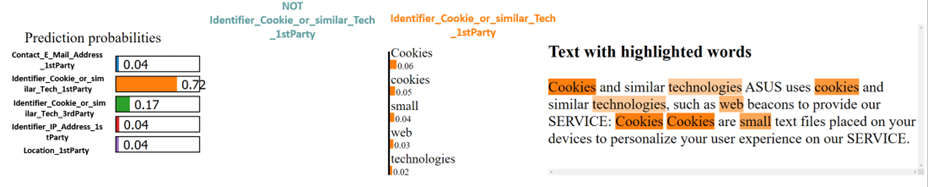
\includegraphics[width=1\linewidth]{figures/explanations_visualisations/section_4a/Picture1.png}
	\caption{Sample visualisation of LIME}   
    \label{fig:lime_sample}
\end{figure}

Explainability techniques should also be distinguished from visualisation techniques (\cite{danilevsky2020}). Explainability techniques are ways to generate the raw mathematical justifications that led to the final explanation presented to the end users. For example, feature importance is one technique that identifies the most important words / phrases in the sentence that led to the prediction, such as LIME. In contrast, visualisation techniques are different ways to present these mathematical justifications to the end user that can deal with how the explanations can be aesthetically presented. One example is a saliency heatmap (such as Figure~\ref{fig:lime_sample}), which highlights the combination of words / phrases that gave rise to the prediction at differing intensities. In this regard, there are also different Python visualisations of LIME. This difference between explainability and visualisation is akin to the difference between proportions and pie charts. While proportions can be presented in pie charts, there is no necessity for this to be so. Proportions can also be presented in a bar chart. Hence, these are two related, but also separate areas of research that go towards the overall objective of explainability.

\subsection{Methodology}
I chose to use LIME because it is model agnostic which allows easy experimentation with different combinations of word representations and models without needing much tweaking. It is also one of the few XAI packages that are easily implementable in Python. In particular, I use the implementation by the LIME creators (\cite{lime_github}). I apply LIME on the different combinations of word representations and models and compare the explainability of LIME's explanations. I presented these explanations to the survey respondents without any amendments to the code output, except for minor editing to the labels in the figure because some labels were cut-off.

\section{Evaluating the effectiveness of XAI methods}
\subsection{Literature review}
There is not much general consensus as to the methods and standards of what makes a particular XAI technique effective. This is because explainability is highly context dependent, as alluded to in Section~\ref{chap1:increasing_opacity}. In terms XAI and the law, the main challenge towards greater adoption of XAI is determining what exactly would be considered sufficiently explainable for legal purposes. While post-hoc methods have been argued to be insufficient to pass muster for non-discrimination law (\cite{vale2022explainable}), it should be noted that legal standards for explainability differ too. What could be insufficiently explainable for non-discrimination law might not apply \textit{mutatis mutandis} to data privacy law under the GDPR (for instance). Indeed, other authors have argued that tort and contract law in medical diagnostics may sometimes mandate using a higher performing model over a more explainable model depending on the specific use case (\cite{hacker2020explainable}). In any case, this capstone makes no claim as to what the applicable standard for explainability is for data privacy, and merely serves as empirical insight as to the perceptions of explainability by potential data subjects.

Apart from the specific requirements of the law, the general field of evaluating XAI is also nascent. Danilevsky et al. provides three categories of evaluating XAI (\cite{danilevsky2020}): First is informal examination of explanation, which are high level discussions of how generated explanations cohere with human intuition. Second is comparison to ground truth, such as quantitative metrics like precision / recall / F1. Third is human evaluation, which is simply to ask humans to evaluate the effectiveness of the explanations. Apart from how XAI is evaluated, what is evaluated includes fidelity (how much the explanation reflect the actual workings of the model), comprehensibility (how easily understood are the explanations), and others. Danilevsky et al. also note that many studies do not state what is being evaluated in XAI assessments. According to Doshi-Velez and Kim, there are few methods to measure human evaluation of XAI as covered in Table~\ref{tab:human_eval_xai}. 

\begin{table}[!ht]
	\resizebox{\textwidth}{!}{%
	\begin{tabular}{|p{0.2\linewidth}|p{0.85\linewidth}|}
	\hline
	\textbf{Method}                 & \textbf{Description}                                                                                                                                        \\ \hline
	Binary forced choice            & Humans are presented with pairs of explanation, and must choose the one that they find of higher quality.                                                   \\ \hline
	Forward simulation / prediction & Humans are presented with an explanation and an input, and must correctly simulate the model's output.                                                      \\ \hline
	Counterfactual simulation       & Humans are presented with an explanation, an input, and an output, and are asked what must be changed to change the model's prediction to a desired output. \\ \hline
	\end{tabular}
	}
	\caption{Methods of measuring human evaluation of XAI. Adapted from (\cite{doshi-velez2017})}
	\label{tab:human_eval_xai}
\end{table}

Further, the purpose of generating the explanation is important towards assessing whether the explanation is effective. Here are some factors which purposes can be categorised into:
\begin{enumerate}
	\item Global vs local: A scientific understanding of a model predicting rainfall would require global explanation since a scientist would be concerned with finding long term correlations, while a consumer who failed to obtain a loan would only require a local explanation to justify why the model made such a prediction.
	\item Area and severity of incompleteness of the problem: For example, a potential buyer of an autonomous vehicle (AV) would have a general curiosity about how they work which requires more inquiry to figure out what aspect of the model to focus on explaining, while a regulator may have specific explanation requirements such as whether the model detects a pedestrian 10 metres before collision.
	\item Time constraints: Consumers that get a bank loan rejected would likely have more time to scrutinise the explanation compared to a compliance manager in the bank who has to process hundreds of claims a day.
	\item Nature of user expertise: A layperson with no training in credit worthiness would not expect details relating to large, complicated models, compared to an auditor that would expect such models to accurately model how human evaluations are made.
\end{enumerate}

Further, as mentioned earlier, there is no agreed upon definition of "explainability". Explainability could be influenced by other value-laden terms, such as trust, effectiveness, fairness, bias, the consequence of making a wrong prediction etc (\cite{rosenfeld2021}). The relative importance of these values and overall requirement of explainability necessarily is dependent on the user of the explanation. All these values are particular important to a data privacy context, as data privacy is a part of the greater legal system. The notion of "rule of law" encompasses these values, and legal systems are judged according to them as well. However, currently, there is also no definitive answer as to how these values linked to explainability can be translated from legal norms to XAI techniques.

It is worth noting that user studies that evaluate post-hoc explanations have been criticised for being inherently flawed because of confirmation bias and that post-hoc explanations may have little to no similarities to how the underlying model made the prediction (\cite{rosenfeld2021}). Nevertheless, since this capstone is concerned only with explaining classical models, similar to LIME's creators, this allow the surrogate model to represent the underlying model's logic fairly well. In any case, as explained below, user studies are not the only method of evaluating XAI in this capstone, so any concerns with user studies can be reduced.

(\cite{gorski2021})
\subsection{Methodology}
Effectiveness of the XAI methods in this capstone are measured in two ways: First it is with regard to ground-truths, as measured by precision / recall / F1 scores. Second is with regard to human evaluation, by using binary forced choice and counterfactual, as well as self-reported metrics related to explainability. These methods attempt to evaluate how explainable LIME methods are when applied onto the different combinations of word representations and models chosen. Further, taking into account Doshi-Velez and Kim's concerns about effectiveness of explanations being evaluated in light of specific purposes, effectiveness is also evaluated across the different potential purposes of the consumer, regulator and software developer that could conceivably arise out of a data privacy context.

(\cite{jasper_evaluating_xai})

(\cite{yalcin2022perceptions})

(\cite{francesca_2021})